%+++++++++++++++++++++++++++++++++++++++++++++++++++++++++++++++
% SUMMARY    : Lecture 9
%            : University of Southern Maine 
%            : @james.quinlan
%            : Ellis Fitzgerald
%+++++++++++++++++++++++++++++++++++++++++++++++++++++++++++++++
\usepackage{tikz} % is Required 
\section*{Objectives}
\begin{outline}
    \1 Regression
    \1 Loss Functions
    \1 Lectures 1-8 Review
    \1 Practice Problems
\end{outline}

\rule[0.0051in]{\textwidth}{0.00025in}
% ----------------------------------------------------------------

\section{Regression}
The previous lectures and materials have mostly covered classification tasks. In general the goal or regression is to predict the labels.  As we know, classification can be binary, where there are two (2) labels: 
\[
y \in \{-1, 1\}
\]

Though, classification tasks can contain $x\mathbb{\in Z^+}$ labels. In a small example, the Iris dataset has three (3) different labels representing the Iris flowers: setosa, versicolor, and virginica.
\[
y \in \{1, 2, 3\}
\]
\textbf{Regression} has the same goal of ``labeling'' features, but not categorically, and instead with real numbers. Regression is a supervised learning technique used to predict continuous outcomes, such as temperature, price, or age, based on input features. For example, predicting the price of a house based on its size and location is a regression task.
\[
y \in \mathbb{R}
\]
For both regression and classification, the dataset takes the same form:
\[
D = \{(x_1, y_1), (x_2, y_2),...,(x_n, y_n)\}
\]
Where for each feature, $x_i$, there is an associated label, $y_i$.

\section{Loss Functions}
\textbf{Loss} is calculated by a function for supervised machine learning tasks. Its responsibility is to answer the question: 
\[
\text{By how much is the model \textit{wrong}?}
\]

\subsection{Zero-to-One Loss}
\textbf{Loss} functions can be simple and binary, similar to classification tasks. For example, a zero-to-one loss function would be denoted as
\[
l_{01} \in \{0, 1\}
\]
In this function, a 1 means the result was incorrect and a 0 means the result matches the anticipated output.

When speaking about loss functions, some may interchangeably call a function's \textbf{Aggregate} (summation) a loss function, but this is more accurately described as being a \textbf{Cost} function.
\[ 
\text{Cost} = \sum_{i=1}^{n} l_{01}(i) = 1 + 0 + 1 + 1 + 0 \ldots
\]
In this cost function, the higher the value the more loss the model has. Simply put: the higher the score $\implies$ the higher the error rate.

\subsection{Absolute Loss}
\textbf{Absolute Loss} takes the actual label associated with the feature $y_i$ and gets the absolute difference with the predicted label value, \footnote{}$\hat{y_i}$.
\footnote[1]{The hat symbol $\hat{}$ implies that this variable is a computed value.}

\[ 
\text{Loss} = |y_i - \hat{y_i}|
\]
\[ 
\text{Cost} = \sum_{i=1}^{n} |y_i - \hat{y_i}|
\]
The downside of the absolute loss function is that it is not \textbf{differentiable}. Recall that differentiable means a derivative exists.

\subsection{Square Loss}
Square loss takes the actual label associated with the feature $y_i$ and squares its difference with the computed $\hat{y_i}$ label value.
\[ 
\text{Loss} = (y_i - \hat{y_i})^2
\]
\[ 
\text{Cost} = \sum_{i=1}^{n} (y_i - \hat{y_i})^2
\]
Because this loss function squares its result, it can be sensitive to outliers. However, it is often preferred over the absolute loss function because it is differentiable.


\subsection{Comparison of Loss Functions}
let's visualize To better understand the characteristics of different loss function and how they behave when the prediction error (the difference between the actual value $y$ and the predicted value $\hat{y}$) varies:

\begin{figure}[h]
\centering
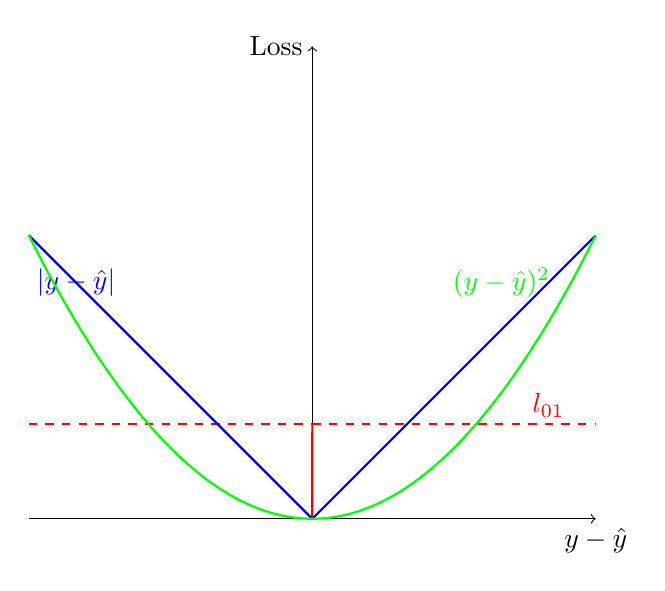
\begin{tikzpicture}[scale=1.2]
    % Grid and axes
    \draw[->] (-3,0) -- (3,0) node[below] {$y - \hat{y}$};
    \draw[->] (0,0) -- (0,5) node[left] {Loss};
    
    % Zero-One Loss
    \draw[thick, red, dashed] (-3,1) -- (-0.001,1);
    \draw[thick, red, dashed] (0.001,1) -- (3,1);
    \draw[thick, red] (-0.001,0) -- (0.001,1);
    \node[red] at (2.5,1.2) {$l_{01}$};
    
    % Absolute Loss
    \draw[thick, blue] (-3,3) -- (0,0) -- (3,3);
    \node[blue] at (-2.5,2.5) {$|y - \hat{y}|$};
    
    % Square Loss
    \draw[thick, green, domain=-3:3, samples=100] plot (\x, {(\x)^2/3});
    \node[green] at (2,2.5) {$(y - \hat{y})^2$};
    
\end{tikzpicture}
\caption{Visual comparison of Zero-One, Absolute, and Square Loss functions}
\label{fig:loss-comparison}
\end{figure}

The figure shows how each loss function behaves differently:
\begin{itemize}
    \item \textbf{Zero-One Loss} (red dashed): Binary output that jumps from 0 to 1 when there is any error
    \item \textbf{Absolute Loss} (blue): Linear increase as error grows, non-differentiable at zero
    \item \textbf{Square Loss} (green): Increases quadratically with error, differentiable everywhere, but more sensitive to outliers than absolute loss
\end{itemize}

\subsection{Objective Function}
Recall that we covered how a \textbf{Cost} function aggregates a \textbf{Loss} function.
\[ 
\text{Cost} = \sum_{i=1}^{n} \text{Loss}
\]
Similarly, there is another function known as the \textbf{Objective Function} which is the sum of the cost and a \textbf{Regularizer}:
\[ 
\text{Objective Function} = \text{Cost} + \text{Regularizer}
\]

The purpose of the regularizer is to discourage large weights by adding a penalty term to the cost function. This helps prevent overfitting and improves generalization. Common regularizers include L1 (Lasso) \cite{tibshirani1996lasso} and L2 (Ridge), which shrink model coefficients during training.

\subsection{Gradient Descent}
Gradient descent \cite{goodfellow2016deep} is essentially a use case for calculating derivatives. In supervised Machine Learning (ML) tasks, its purpose is to find global minima (where the derivative is 0) to optimize a model's loss function. %

Here are the names of some notable gradient descent methods:
\begin{outline}
    \1 \textbf{Vanilla} — The basic form of gradient descent where the entire dataset is used to compute the gradient in each iteration. \textit{Use: simple and stable for small datasets.}
    \1 \textbf{Stochastic} — Uses a single random data point to update the weights in each iteration. \textit{Use: faster updates and more noise, good for large datasets.}
    \1 \textbf{Minibatch} — Uses a small batch of data points to compute the gradient. \textit{Use: balances stability and speed, commonly used in practice.}
    \1 \textbf{Hessian} — Refers to second-order optimization using the Hessian matrix of second derivatives. \textit{Use: captures curvature for more accurate updates but is computationally expensive.}
    \1 \textbf{Momentum} — Accelerates gradient descent by adding a fraction of the previous update to the current one. \textit{Use: helps escape local minima and smoothens convergence.}
\end{outline}


\subsubsection{Learning Rate}
Gradient descent performance depends heavily on the learning rate, which determines the size of steps taken during optimization. A good starting point is often 0.01 or 0.001:
\begin{itemize}
    \item Too large: Overshoots minima.
    \item Too small: Slow convergence.
\end{itemize}

% ----------------------------------------------------------------
\section{Lectures 1-7 Review}

\subsection{The Perceptron\cite{rosenblatt1958perceptron}}
\begin{outline}
    \1 Developed by \textbf{Rosenblatt} in \textbf{1957} at Cornell University
    \1 It was the first "AI" algorithm
    \1 \textbf{Binary Classification} Task
    \1 The goal is to find \textit{a} hyperplane (seperating the data)
    \1 Assumes data is \textbf{Linearly Separable}
    \1 Calculates weight vector $\vec{w}$ and bias $b$ 
    \1 ``Bundle \& Save'': This trick will save time by removing the need to calculate $b$. We do this by ``bundling" $b$ into $\vec{w}$: 
    \begin{align*}
    \vec{w} &= \begin{bmatrix}
           w_{1}    \\
           w_{2}    \\
           \vdots   \\
           w_{p}    \\
           b        \\
         \end{bmatrix} \\
    \end{align*}
    \1 $\vec{w} \in \mathcal{H}$ where $\mathcal{H}$ is the \textbf{Decision Boundary} or \textbf{Hyperplane}
\end{outline}

\[
\mathcal{H} = \{\vec{x} | \vec{w}^T\vec{x} + b = 0\}
\]

\subsection{KNN\cite{guo2003knn}}
\begin{outline}
    \1 Stands for \textbf{$k$ Nearest Neighbors}
    \1 Loops over all neighbors and calculates distance
    \1 Assumes there is a pattern
    \1 Not designed for data with random values
    \1 Sorts distances and returns $k$ nearest
    \1 \textbf{Regression:} Averages values to nearest neighbor values
    \1 \textbf{Classification:} Sets label to the mode of nearest neighbor values
\end{outline}

\begin{verbatim}
w = 0
m = 1
while m > 0:
    m = 0
    for i = 1..n:
        if y[i] * dot(w, x[i]) <= 0:
            w = w + alpha * y[i] * x[i]
            m = m + 1
        end
    end
end
\end{verbatim}

% ----------------------------------------------------------------
\section{Practice Problems}
\begin{outline}[enumerate]
    \1 What is the benefit of having fewer dimensions, features, or components in your vectors? \\
    \textit{Answer:} Reducing dimensions helps prevent overfitting, speeds up computation, and improves generalization.
    
    \1 What are the different types of Supervised ML? \\
    \textit{Answer:} Classification and Regression.
    
    \1 What is a loss function? \\
    \textit{Answer:} A function that measures how far off the model’s predictions are from the actual labels.
    
    \1 What is KNN? How could it be used differently for both Classification and Regression? \\
    \textit{Answer:} KNN is a neighbor-based method that can predict by majority vote (classification) or by averaging (regression).
    
    \1 What does SVM stand for? What is its purpose? \\
    \textit{Answer:} Support Vector Machine; used to find an optimal separating hyperplane between classes.
    
    \1 What is the definition of a distance function? Give examples. \\
    \textit{Answer:} A distance function measures how far apart points are. Examples: Euclidean distance, Manhattan distance.
\end{outline}

\bibliographystyle{plain}
